\documentclass[10pt,a4paper]{article}
\usepackage[utf8x]{inputenc}
\usepackage{ucs}
\usepackage[left=2.00cm, right=2.00cm, top=2.00cm, bottom=2.00cm]{geometry}
\renewcommand\familydefault{\sfdefault}

\title{Robotics - WS1819}
\author{}
\date{2018}

%math
\usepackage{amsmath}
\usepackage{amsfonts}
\usepackage{amssymb}
\usepackage{amstext}
\usepackage{mathtools}

%graphics
\usepackage{graphicx}
\usepackage{floatflt}
\usepackage{float}

%tabular
\usepackage{tabularx}
\usepackage[font=small,labelfont=small]{caption}
\usepackage{colortbl}
\usepackage[dvipsnames]{xcolor}
%\renewcommand{\arraystretch}{2}
%\arrayrulecolor{white}

%tikz
\usepackage{tikz}
\usetikzlibrary{shapes, petri}
\tikzstyle{ell}=[ellipse,draw, yshift=-2mm]
\tikzstyle{rec} = [rectangle, draw]
\tikzstyle{dia} = [diamond, aspect=2, draw, yshift=-5mm]
\tikzstyle{cir} = [circle, draw, minimum size=3mm]
\tikzstyle{arrHV} = [to path={-| (\tikztotarget)}]
\tikzstyle{arrVH} = [to path={|- (\tikztotarget)}]
\tikzstyle{whileright} = [xshift=20mm, yshift=-3mm]
\tikzstyle{whileleft} = [xshift=-20mm, yshift=-3mm]
\tikzstyle{txtright} = [above, xshift=15mm]
\tikzstyle{txtleft} = [above, xshift=-15mm]
\tikzstyle{empty} = [coordinate]
\usetikzlibrary{positioning}

%listings
\usepackage{listings}
\lstdefinestyle{costum} {
	language=Bash,
	basicstyle=\footnotesize\ttfamily,
	keywordstyle=\bfseries\color{cyan!50!blue},
	commentstyle=\itshape\color{black!50},
	%identifierstyle=\color{blue},
	stringstyle=\color{green!50!black},
	morekeywords={returns, loop, each}
}
\lstset{style=costum}


%costum layout
\setlength{\parindent}{0cm}
\usepackage{fancyhdr}
\usepackage{xcolor}
\pagestyle{fancy}
\fancyhf{}
\fancyhead[L]{
	\strut\rlap{\color{orange!50!black}\rule[-\dp\strutbox]{\headwidth}{\headheight}}
	\textcolor {white} {Summary: Robotics}}
\fancyfoot[L]{
	\strut\rlap{\color{orange!50!black}\rule[-\dp\strutbox]{\headwidth}{\headheight}}
	\textcolor {white} {last changed: \today}}
\fancyhead[R]{\textcolor{white}{Winter semester 2018/19}}
%\lfoot{}
\fancyfoot[R]{\textcolor{white} {\thepage}}
%\renewcommand{\footrulewidth}{1pt}

%multicol
\usepackage{multicol}
%\setlength{\columnseprule}{0pt}
%\setlength{\columnsep}{20.0pt}



%custom title color
\usepackage{titlesec}
%\titleformat{\section}
%{\color{cyan!80!blue}\normalfont\Large\bfseries}
%{\color{black}\thesection}{1em}{}

%\titleformat{\subsubsection}
%{\color{blue!30!black!70}\normalfont\bfseries}
%{\color{black}\thesection}{1em}{}

\setcounter{secnumdepth}{4}

%\titleformat{\paragraph}
%{\color{green!30!black!70}\normalfont\normalsize\bfseries}{\theparagraph}{1em}{}
%\titlespacing*{\paragraph}
%{0pt}{3.25ex plus 1ex minus .2ex}{1.5ex plus .2ex}

%tab
\newcommand{\tab}[1][1]{\hspace*{#1cm}}

%color_summary
\newcommand{\sumcolor}[1]{\textcolor{red!10!green!40!blue}{#1}}

%coloring
\newcommand{\redr}{\textcolor{red}{r}}
\newcommand{\greeng}{\textcolor{green}{g}}
\newcommand{\blueb}{\textcolor{blue}{b}}

%other
\usepackage{enumerate}

%hyperref
\usepackage{hyperref}

%vector
\newcommand{\vect}[1]{\ensuremath{\begin{bmatrix}#1\end{bmatrix}}}

%other
\newcommand{\atan}{\ensuremath{\mathrm{atan2 }}}
\newcommand{\add}{\textcolor{red}{ADD \\}}
\newcommand{\maybe}{\textcolor{red}{MAYBE \\}}


%Geprüft:
%Coordinate Frames
%Forward Kinematics
%Inverse Kinematics
%Jacobians
%Dynamics
%Trajectories
%Manipulator-mechanics design
%Linear Control
%Nonlinear Control
%Force control

%TODO
%rotation about x, y and z expressed by rotation matrices


\begin{document}
	
\section{Coordinate Frames}
\subsection{Descriptions}

\subsubsection{Description of a position}
Let $A$ be a defined coordinate system in addition to the universe coordinate system and $P$ a position vector. Then \\
\begin{equation*}
^AP = \vect{p_x \\ p_y \\ p_z} \\
\end{equation*}
is a point represented as a vector in the coordinate system $\{A\}$ ($p_x$, $p_y$ and $p_z$ indicate distances along the axes of $\{A\}$)


\subsubsection{Description of an orientation}
Let $\{A\}$ and $\{B\}$ be frames and \\
The rotation matrix which describes $\{B\}$ relative to $\{A\}$ is defined as:
\begin{equation*}
_B^AR := ~^B_AR^T = ~^B_AR^{-1} = \begin{bmatrix}
r_{11} & r_{12} & r_{13} \\
r_{21} & r_{22} & r_{23} \\
r_{31} & r_{32} & r_{33} \\
\end{bmatrix} = \begin{bmatrix}
\hat{X}_B ⋅ \hat{X}_A & \hat{Y}_B ⋅ \hat{X}_A & \hat{Z}_B ⋅ \hat{X}_A \\
\hat{X}_B ⋅ \hat{Y}_A & \hat{Y}_B ⋅ \hat{Y}_A & \hat{Z}_B ⋅ \hat{Y}_A \\
\hat{X}_B ⋅ \hat{Z}_A & \hat{Y}_B ⋅ \hat{Z}_A & \hat{Z}_B ⋅ \hat{Z}_A \\
\end{bmatrix}
\end{equation*}

\subsubsection{Description of a frame}
Let $\{A\}$ be a coordinate system, and \\
let $^A_BR$ a rotation matrix that describes $\{B\}$ relative to $\{A\}$, and \\
let $^AP_{BORG}$ be a vector that locates the origin of $\{B\}$ relative to $\{A\}$. \\
The frame $\{B\}$ is defined as:
\begin{equation*}
\{B\} := \{~^A_BR, ~^AP_{BORG}\}
\end{equation*}

\subsection{Mapping of frames}
Let $\{A\}$ and $\{B\}$ be frames and\\
$^A_BR$ a rotation matrix that describes $\{B\}$ relative to $\{A\}$. \\
Let $^AP_{BORG}$ be a vector that locates the origin of $\{B\}$ relative to $\{A\}$. \\
Let $^BP$ be a vector that locates a point P relative to $\{B\}$. \\
Then this point relative to $\{A\}$ is defined as:
\begin{equation*}
^AP := ~^A_BR ⋅ ~^BP + ~^AP_{BORG}
\end{equation*}
\begin{equation*}
\vect{^AP \\ 1} = \left[\begin{array}{c|c}
^A_BR & ^AP_{BORG} \\ \hline 0~ 0~ 0 & 1
\end{array}\right] ⋅ \vect{^BP \\ 1}
\end{equation*}
\begin{equation*}
^AP =~ ^A_BT ⋅~^BP
\end{equation*}

\subsection{Transformation arithmetic}
\subsubsection{Compound transformations}
Let $^A_BT$ and $^B_CT$ be homogeneous transforms. \\
Then $^A_CT$ is defined as: \\
$$
^A_CT := ~^A_BT ⋅~ ^B_CT = \left[\begin{array}{c|c}
^A_BR ⋅~^B_CR & ^A_BR ⋅~^BP_{CORG} + ~^AP_{BORG} \\
\hline
0 ~0 ~0 & 1
\end{array}\right]
$$

\subsubsection{Inverting a transform}
Let $^A_BT$ be a transform. \\
Then $^B_AT$ is defined as: \\
$$
^B_AT := ~^A_BT^{-1} = \left[\begin{array}{c|c}
^A_BR^T & -^A_BR^T ⋅~^AP_{BORG} \\
\hline
0 ~0 ~0 & 1
\end{array}\right]
$$

\section{Forward Kinematics}
\subsection{Joints}
\begin{itemize}
	\item Revolute/Rotational/Revolving/"wisting joint: $\Delta \theta$
	\item Prismatic/Linear joint: $\Delta x$
	\item Helical/Screw/Cylindrical joint: $\Delta x, \Delta \theta$
	\item Spherical joint: $\Delta \theta, \Delta \phi, \Delta \psi$
	\item Flat/Planar joint: $\Delta x, \Delta y, \Delta \theta$
\end{itemize}

\subsection{Denavit-Hartenberg}
\subsubsection{Attach a frame to a link} 
Let link $i$ be a link with two axes Axis $i$ and Axis ${i+1}$ and the link length $a_i$. \\
The frame $\{i\}$ will be located on the link as follows:
\begin{description}
	\item The $\hat{Z}$-axis of frame $\{i\}$ is called $\hat{Z}_i$ and is coincident with the Axis $i$
	\item The origin of frame $\{i\}$ is located where the $a_i$ orthogonal intersects the Axis $i$
	\item The $\hat{X}$-axis of frame $\{i\}$ is called $\hat{X}_i$ and points along $a_i$ in the direction from Axis $i$ to Axis $i+1$
	\item The link twist $\alpha_i$ is measured in the right-hand sense about $\hat{X}_i$
	\item The $\hat{Y}$-axis of frame $\{i\}$ is called $\hat{Y}_i$ and is formed by the right-hand rule
\end{description}

\subsubsection{Link-Frame Attachment Procedure}
\begin{enumerate}
	\item Identify the joint axes and imagine (or draw) infinite lines along them. steps 2 through 5 below, consider two of these neighboring lines (at axes $i$ and $i + 1$).
	\item Identify the common perpendicular between them, or point of intersection. At the point of intersection, or at the point where the common perpendicular meets the $i$-th axis, assign the link-frame origin. 
	\item Assign the $\hat{Z}_i$ axis pointing along the $i$-th joint axis. 
	\item Assign the $\hat{X}_i$ axis pointing along the common perpendicular, or, if the axes intersect, assign $\hat{X}_i$ to be normal to the plane containing the two axes. 
	\item Assign the $\hat{Y}_i$ axis to complete a right-hand coordinate system. 
	\item Assign $\{0\}$ to match $\{1\}$ when the first joint variable is zero. For $\{N\}$, choose an origin location and $\hat{X}_N$ direction freely, but generally so as to cause as many linkage parameters as possible to become zero.
\end{enumerate}

\subsubsection{Denavit-Hartenberg notation}
Let $a_{i-1}$ be the link length from link $i-1$ to $i$, and \\
let $\alpha_i$ be the link twist from axis $i-1$ to $i$ (right-hand sense), and \\
let $d_i$ be the link offset from link $i-1$ to $i$, and \\
let $\theta_i$ be the joint angle of a rotation about the common axes of link $i-1$ and $i$ (right-hand sense). \\
It follows: 
$$
	\begin{array}{|c|c|c|c|c|}
	\hline
	i & a_{i-1} & \alpha_{i-1} & d_i & \theta_i \\
	\hline
	\hline
	1 & 0 & 0 & d_1 & \theta_1 \\
	\hline
	2 &  a_1 & \alpha_1 & d_2 & \theta_2 \\
	\hline
	\multicolumn{5}{|c|}{\vdots} \\
	\hline
	n & a_{n-1} & \alpha_{n-1} & d_n & \theta_n \\
	\hline
	\end{array}
$$

\subsubsection{Link parameters in terms of the link frames}
$$
a_i = \text{the distance from } \hat{Z}_i \text{ to } \hat{Z}_{i+1} \text{ measured along } \hat{X}_i
$$
$$
\alpha_i = \text{the angle from } \hat{Z}_i \text{ to } \hat{Z}_{i+1} \text{ measured about } \hat{X}_i
$$
$$
d_i = \text{the distance from } \hat{X}_{i-1} \text{ to } \hat{X}_i \text{ measured along } \hat{Z}_i
$$
$$
\theta_i = \text{the angle from } \hat{X}_{i-1} \text{ to } \hat{X}_i \text{ measured about } \hat{Z}_i
$$

\subsection{Forward Kinematics}
\subsubsection{Link transformations}
Let $a_{i-1}$ be the link length from link $i-1$ to $i$, and \\
let $\alpha_i$ be the link twist from axis $i-1$ to $i$ (right-hand sense), and \\
let $d_i$ be the link offset from link $i-1$ to $i$, and \\
let $\theta_i$ be the joint angle of a rotation about the common axes of link $i-1$ and $i$ (right-hand sense). \\
The transform that defines frame $\{i\}$ relative to frame $\{i-1\}$ is calculated as: \\
$$
	^{i-1}_iT = \begin{bmatrix}
	\cos \theta_i & -\sin \theta_i & 0 & a_{i-1} \\
	\sin \theta_i \cos \alpha_{i-1} & \cos \theta_i \cos \alpha_{i-1} & -\sin \alpha_{i-1} & -\sin \alpha_{i-1} d_i \\
	\sin \theta_i \sin \alpha_{i-1} & \cos \theta_i \sin \alpha_{i-1} & \cos \alpha_{i-1} & \cos \alpha_{i-1} d_i \\
	0 & 0 & 0 & 1		
	\end{bmatrix}
$$

\subsubsection{Concatenating link transformations}

Let $^{i-1}_iT$ be the transform that defines frame $\{i\}$ relative to frame $\{i-1\}$ and let frame $\{0\}$ be the first frame and $\{N\}$ be the last frame. \\
$^0_NT$ is calculated as:
$$
^0_NT = ~^0_1T ⋅ ~^1_2T ⋅ \dots ⋅ ~^{N-1}_NT
$$

\subsubsection{Forward Kinematics of a planar manipulator}
Let be given a manipulator with n joints, and \\
Let all joints be parallel, and \\
let the joint variable of the $i$-joint be $\theta_i$.
It follows:
$$
^{i-1}_iT = \begin{bmatrix}
\cos \theta_i & -\sin \theta_i & 0 & a_{i-1} \\
\sin \theta_i & \cos \theta_i & 0 & 0 \\
0 & 0 & 1 & 0 \\
0 & 0 & 0 & 1		
\end{bmatrix}
$$

$$
^0_nR = \begin{bmatrix}
\cos(\theta_1 + \dots + \theta_n) & -\sin(\theta_1 + \dots + \theta_n) & 0 \\
\sin(\theta_1 + \dots + \theta_n) & \cos(\theta_1 + \dots + \theta_n) & 0 \\
0 & 0 & 1
\end{bmatrix}
$$

(The orientation of the frame $\{n\}$ can be described using only one angle $\theta = \theta_1 + \dots + \theta_n$)

$$
^0P_{nORG} = ~^0P_{1ORG} + ~^0_1R ⋅ ~^1P_{2ORG} + ~^0_2R ⋅ ~^2P_{3ORG} + \dots + ~^0_{n-1}R ⋅ ~^{n-1}P_{nORG} = ~^0P_{1ORG} + \sum_{i = 2}^{n} ~^0_{i-1}R ⋅ ~^{i-1}P_{iORG}
$$

$$
^{0}_{n+1}T = \begin{bmatrix}
	\cos(\theta_1 + \dots + \theta_n) & -\sin(\theta_1 + \dots + \theta_n) & 0 & a_1 ⋅ \cos(\theta_1) + a_2 ⋅ \cos(\theta_1 + \theta_2) + \dots + l_n ⋅ \cos(\theta_1 + \dots + \theta_n) \\
	\sin(\theta_1 + \dots + \theta_n) & \cos(\theta_1 + \dots + \theta_n) & 0 & a_1 ⋅ \sin(\theta_1) + a_2 ⋅ \sin(\theta_1 + \theta_2) + \dots + l_n ⋅ \sin(\theta_1 + \dots + \theta_n) \\
	0 & 0 & 1 & 0 \\
	0 & 0 & 0 & 1		
\end{bmatrix}
$$	


\subsection{Frames With Standard Names}
\begin{itemize}
	\item Base Frame $\{B\}$
	\item Station Frame $\{S\}$
	\item Wrist Frame $\{W\}$
	\item Tool Frame $\{T\}$
	\item Goal Frame $\{G\}$
\end{itemize}


\section{Jacobians: velocities and static forces}
\subsection{Linear Velocity}
Let $^BQ$ be a position vector relative to frame $\{B\}$. \\
The velocity of $Q$ relative to frame $\{B\}$ is computed as the derivative of $^BQ$ w.r.t. time and defined as:
$$
^BV_Q = \frac{d}{dt} ~^BQ
$$

Let $^UCORG$ be the origin of frame $\{C\}$ relative to frame $\{U\}$ \\
The velocity of $^UCORG$ relative to the universe frame $\{U\}$ is defined as:
$$
v_C = ~^UV_{CORG}
$$

and the velocity vector of $^UCORG$ expressed int terms of frame $\{A\}$ (though differentiation done relative to $\{U\}$) is defined as:
$$
^Av_C = ~^A_UR ⋅ v_C
$$

\subsection{Angular Velocity}
Let $\{A\}$ and $\{B\}$ be two frames. \\
The angular velocity of a rotation of frame $\{B\}$ relative to $\{A\}$ is defined as:
$$
^A\Omega_B
$$
, where the direction of $^A\Omega_B$ indicates the axis of rotation \\
and the magnitude of $^A\Omega_B$ indicates the speed of rotation \\

Let $\{C\}$ be a frame and $\{U\}$ be the universe frame \\
The angular velocity of a rotation of frame $\{C\}$ relative to $\{U\}$ is defined as:
$$
\omega_C = ~^U\Omega_{C}
$$

and the angular velocity vector of $\{C\}$ relative to $\{U\}$ expressed in terms of frame $\{A\}$ is defined as:
$$
^A\omega_C
$$

\subsection{Transformation of velocities}
Let $\{A\}$ and $\{B\}$ be two frames \\
Let $^BQ$ be a position vector relative to $\{B\}$ which may change with time \\
Let the location of $\{B\}$ relative to $\{A\}$ be described by a position vector $^AP_{BORG}$ which may change with time \\
Let $^A\Omega_B$ be a vector describing the rotational velocity of $\{B\}$ relative to $\{A\}$ \\
Let $^A_BR$ a rotation matrix describing $\{B\}$ relative to $\{A\}$ \\
The velocity of $Q$ relative to $\{A\}$ is computed as: \\
$$
^AV_Q = ~^AV_{BORG} + ~^A_BR ⋅~^BV_Q + ~^A\Omega_B \times ~^A_BR ⋅ ~^BQ
$$

\subsection{Velocity "Propagation" from link to link}
\subsubsection{Rotational joints}
Let joint $i+1$ be rotational: \\

Let $^{i+1}_iR$ a rotation matrix describing $\{i\}$ relative to $\{i+1\}$ \\
Let $^i\omega_i$ be the angular velocity vector of link $\{i\}$ relative to $\{B\}$ expressed in terms of frame $\{i\}$ \\
The angular velocity of link $i + 1$ with respect to frame $\{i + 1\}$ is calculated as:
$$
^{i+1}\omega_{i+1} = ~^{i+1}_iR ⋅ ~^i\omega_i + \dot \theta_{i+1} ⋅ ~^{i+1}\hat{Z}_{i+1}
$$
, where $\dot \theta_{i+1} ⋅ ^{i+1}\hat{Z}_{i+1} = ~^{i+1}\vect{0 \\ 0 \\ \dot{\theta}_{i+1}}$ \\
\\

Let $^{i+1}_iR$ a rotation matrix describing $\{i\}$ relative to $\{i+1\}$ \\
Let $^iv_i$ be the linear velocity of the origin of link $\{i\}$ relative to $\{B\}$ expressed in terms of frame $\{i\}$ \\
Let $^i\omega_i$ be the angular velocity vector of link $\{i\}$ relative to $\{B\}$ expressed in terms of frame $\{i\}$ \\
Let $^iP_{i+1}$ be the origin of $\{i+1\}$ relative to $\{i\}$
The linear velocity of link $i + 1$ with respect to frame $\{i + 1\}$ is calculated as:
$$
^{i+1}v_{i+1} = ~^{i+1}_iR(^iv_i + ~^i\omega_i \times ~^iP_{i+1})
$$

\subsubsection{Prismatic joints}
Let joint $i+1$ be prismatic: \\

Let $^{i+1}_iR$ a rotation matrix describing $\{i\}$ relative to $\{i+1\}$ \\
Let $^i\omega_i$ be the angular velocity vector of link $\{i\}$ relative to $\{B\}$ expressed in terms of frame $\{i\}$ \\
The angular velocity of link $i + 1$ with respect to frame $\{i + 1\}$ is calculated as:
$$
^{i+1}\omega_{i+1} = ~^{i+1}_iR ⋅ ~^i\omega_i
$$

Let $^{i+1}_iR$ a rotation matrix describing $\{i\}$ relative to $\{i+1\}$ \\
Let $^iv_i$ be the linear velocity of the origin of link $\{i\}$ relative to $\{B\}$ expressed in terms of frame $\{i\}$ \\
Let $^i\omega_i$ be the angular velocity vector of link $\{i\}$ relative to $\{B\}$ expressed in terms of frame $\{i\}$ \\
Let $^iP_{i+1}$ be the origin of $\{i+1\}$ relative to $\{i\}$
The linear velocity of link $i + 1$ with respect to frame $\{i + 1\}$ is calculated as:
$$
^{i+1}v_{i+1} = ~^{i+1}_iR(^iv_i + ~^i\omega_i \times ~^iP_{i+1}) + \dot{d}_{i+1} ⋅ ~^{i+1}\hat{Z}_{i+1}
$$

\subsection{Jacobians}
\subsubsection{Jacobian-Matrix}
Let $p(\Theta) = \vect{p_1 \\ p_2 \\ p_3}$ be a position vector.
The Jacobian is computed as: \\
$$
^i\mathcal{J}(\Theta) = \begin{bmatrix}
\frac{\partial p_1}{\partial \theta_1} & \dots & \frac{\partial p_1}{\partial \theta_n} \\
\frac{\partial p_2}{\partial \theta_1} & \dots & \frac{\partial p_2}{\partial \theta_n} \\
\frac{\partial p_3}{\partial \theta_1} & \dots & \frac{\partial p_3}{\partial \theta_n} \\
^0Z_1 & \dots & ^0Z_n
\end{bmatrix}
$$
, with $\Theta = \vect{\theta_1 \\ \vdots \\ \theta_n}$



\subsubsection{Relate Joint Velocities to Cartesian Velocities}
$$
^i\nu = \vect{^iv \\ ^i\omega} = ~^i\mathcal{J}(\Theta) ⋅ \dot{\Theta}
$$
$$
	\dot{\Theta} = ~^i\mathcal{J}^{-1}(\Theta) ⋅ ~^i\nu
$$
, where $^i\nu$ is a vector of Cartesian velocities (here: of the end-effector frame relative to $\{B\}$): A linear velocity vector expressed in terms of $\{i\}$ and a rotational velocity vector expressed in $\{i\}$. and \\
$\Theta = \vect{\theta_1 \\ \vdots \\ \theta_n}$ \\

Dimension of the Jacobian Matrix:
\begin{itemize}
	\item Number of rows $\hat{=}$ Number of degrees of freedom in the Cartesian space ($\times 2$ for velocity and angular velocity)
	\item Number of columns $\hat{=}$ Number of joints of the manipulator
\end{itemize}

\subsubsection{Changing a Jacobian's frame of reference}
Let $^B\mathcal{J}(\Theta)$ be a Jacobian written in frame $\{B\}$ (with $^B\nu  = ~^B\mathcal{J}(\Theta)\dot \Theta$)\\
The Jacobian written in $\{A\}$ is computed as: \\
$$
^A\mathcal{J}(\Theta) = \left[\begin{array}{c|c}
^A_BR & 0 \\
\hline
0 & ^A_BR
\end{array}\right] ⋅ ~^B\mathcal{J}(\Theta)
$$

\subsection{Singularity}
\subsubsection{Categories}
\begin{itemize}
	\item \textbf{Workspace-boundary singularities} occur when the manipulator is fully stretched out or folded back on itself in such a way that the end-effector is at or very near the boundary of the workspace
	\item \textbf{Workspace interior singularities} occur away from the workspace boundary; they generally are caused by a lining up of two or more joint axes
\end{itemize}

\subsubsection{Calculation}
Let $\mathcal{J}(\Theta)$ be a Jacobian (with $v  = \mathcal{J}(\Theta)\dot \Theta$)\\
The Jacobian is singular (a singularity of the mechanism exists) if: \\
$$
\det[\mathcal{J}(\Theta)] = 0
$$

\subsection{Static Forces in Manipulators}
Let $^{i+1}_iR$ be a rotation matrix describing $\{i\}$ relative to $\{i+1\}$ and\\
let $^{i+1}f_{i+1}$ be a force exerted on link $i+1$ by link $i$ relative to link $i+1$ \\
The force exerted on link $i$ by link $i-1$ relative to link $i$ is defined as:
$$
^if_i = ~^i_{i+1}R ⋅ ~^{i+1}f_{i+1}
$$ \\

Let $^{i+1}_iR$ be a rotation matrix describing $\{i\}$ relative to $\{i+1\}$ and\\
let $^{i+1}n_{i+1}$ be a torque exerted on link $i+1$ by link $i$ relative to link $i+1$ and \\
let $^iP_{i+1}$ be the origin of frame $\{i+1\}$ relative to $\{i\}$ \\
The torque exerted on link $i$ by link $i-1$ relative to link $i$ is defined as:
$$
^in_i = ~^i_{i+1}R ⋅ ~^{i+1}n_{i+1} + ~^iP_{i+1} \times ~^if_i
$$

\subsubsection{Calculate the joint Torque required to maintain the static equilibrium}
\paragraph{Rotational joints:} ~\\
Let $^in_i$ be the torque exerted on link $i$ by link $i-1$ relative to link $i$ and\\
let $^i\hat{Z}_i$ be the joint axis vector. \\
The joint torque required to maintain the static equilibrium is computed as:
$$
\tau_i = ~^in_i^T ⋅ ~^i\hat{Z}_i
$$

\paragraph{Prismatic joints:} ~\\
Let $^if_i$ be the force exerted on link $i$ by link $i-1$ relative to link $i$ and\\
let $^i\hat{Z}_i$ be the joint axis vector. \\
The joint torque required to maintain the static equilibrium is computed as:
$$
\tau_i = ~^if_i^T ⋅ ~^i\hat{Z}_i
$$

\subsection{Jacobians in the Force Domain}
Let $\mathcal{J}$ be a Jacobian (with $\nu  = \mathcal{J}(\Theta)\dot \Theta$) expressed in terms of $\{0\}$ and \\
let $\mathcal{F}$ be a $6 \times 1$ Cartesian force-moment vector acting at the end-effector expressed in terms of $\{0\}$ ($\mathcal{F} = [F, N]^T$ and $F$ is the force acting on the center of the mass of the link and $N$ is the moment acting on the center of the mass of the link)\\
The vector of torques at the joints is calculated as:
$$
\tau = ~^0\mathcal{J}^T ⋅ ~^0\mathcal{F}
$$

\section{Dynamics}
\subsection{Acceleration of a rigid body}
Let $^BV_Q$ the velocity of a point $Q$ relative to $\{B\}$ \\
The linear acceleration of $Q$ relative to $\{B\}$ is defined as:
$$
^B\dot V_Q = \frac d {dt} ~^BV_Q
$$
\\

Let $^A\Omega_B$ be the angular velocity of a rotation of frame $\{B\}$ relative to $\{A\}$ \\
The angular acceleration of $\{B\}$ relative to $\{A\}$ is defined as:
$$
^A\dot \Omega_B = \frac d {dt} ~^A\Omega_B
$$
\\

Let $^UAORG$ be the origin of frame $\{A\}$ relative to frame $\{U\}$ \\
The acceleration of $^UAORG$ relative to the universe frame $\{U\}$ is defined as:
$$
\dot v_A = ~^U\dot V_{AORG}
$$
\\

Let $\{A\}$ be a frame and $\{U\}$ be the universe frame \\
The angular acceleration of a rotation of frame $\{A\}$ relative to $\{U\}$ is defined as:
$$
\dot \omega_A = ~^U \dot \Omega_{A}
$$

\subsubsection{Linear acceleration} \maybe
Let $^BQ$ be a position vector relative to frame $\{B\}$ and \\
let $^B\dot V_Q$ be the linear acceleration of $Q$ relative to $\{B\}$ and \\
let $^B V_Q$ be the linear velocity of $Q$ relative to $\{B\}$ and \\
let $^A\dot \Omega_B$ be a vector describing the angular acceleration of $\{B\}$ relative to $\{A\}$ and \\
let $^A\Omega_B$ be a vector describing the angular velocity of $\{B\}$ relative to $\{A\}$ \\
The linear acceleration of a position vector $Q$ relative to $\{A\}$ is calculated as:
$$
^A\dot V_Q = ~^A\dot{V}_{BORG} + ~^A_BR ⋅ ~^B\dot V_Q + 2 ⋅ ~^A\Omega_B \times ~^A_BR ⋅ ~^BV_Q + ~^A\dot \Omega_B \times ~^A_BR ⋅ ~^BQ + ~^A\Omega_B \times (^A\Omega_B \times ~^A_BR ⋅ ~^BQ)
$$
\\
in the case of $^BV_Q = ^B\dot{V}_Q = 0$:
$$
^A\dot V_Q = ~^A\dot{V}_{BORG} + ~^A\dot \Omega_B \times ~^A_BR ⋅ ~^BQ + ~^A\Omega_B \times (^A\Omega_B \times ~^A_BR ⋅ ~^BQ)
$$

\subsubsection{Angular acceleration} \maybe
Let $^A\Omega_B$ be a vector describing the angular velocity of $\{B\}$ relative to $\{A\}$ and \\
let $^A\dot \Omega_B$ be the vector describing the angular acceleration of $\{B\}$ relative to $\{A\}$ and \\
let $^B\Omega_C$ be a vector describing the angular velocity of $\{C\}$ relative to $\{B\}$ and \\
let $^B\dot \Omega_C$ be the vector describing the angular acceleration of $\{C\}$ relative to $\{B\}$ \\
The angular acceleration of a rotation of $\{C\}$ relative to $\{A\}$ is defined as:
$$
^A\dot \Omega_C = ~^A\dot \Omega_B + ~^A_BR ⋅ ~^B \dot \Omega_C + ~^A\Omega_B \times ~^A_BR ⋅ ~^B\Omega_C
$$

\subsection{Acceleration from link to link}
\subsubsection{Rotational joints}
Let joint $i+1$ be rotational: \\

Let $^i\omega_i$ be the angular velocity vector of link $\{i\}$ relative to $\{B\}$ expressed in terms of frame $\{i\}$ \\
Let $^i\dot\omega_i$ be the angular acceleration vector of link $\{i\}$ relative to $\{B\}$ expressed in terms of frame $\{i\}$ \\
The angular acceleration of link $i + 1$ with respect to frame $\{i + 1\}$ is calculated as:
$$
^{i+1}\dot \omega_{i+1} = ~^{i+1}_iR ⋅ ~^i\dot \omega_i + ~^{i+1}_iR ⋅ ~^i\omega_i \times \dot \theta_{i+1} ⋅ ~^{i+1}\hat{Z}_{i+1} + \ddot \theta_{i+1} ⋅ ~^{i+1}\hat{Z}_{i+1}
$$
, where $\ddot \theta_{i+1} ⋅ ^{i+1}\hat{Z}_{i+1} = ~^{i+1}\vect{0 \\ 0 \\ \ddot{\theta}_{i+1}}$ \\
\\

Let $^i\dot v_i$ be the linear acceleration of the origin of link $\{i\}$ relative to $\{B\}$ expressed in terms of frame $\{i\}$ \\
Let $^i\omega_i$ be the angular velocity vector of link $\{i\}$ relative to $\{B\}$ expressed in terms of frame $\{i\}$ \\
Let $^i\dot \omega_i$ be the angular acceleration vector of link $\{i\}$ relative to $\{B\}$ expressed in terms of frame $\{i\}$ \\
Let $^iP_{i+1}$ be the origin of $\{i+1\}$ relative to $\{i\}$
The linear acceleration of link $i + 1$ with respect to frame $\{i + 1\}$ is calculated as:
$$
^{i+1}\dot v_{i+1} = ~^{i+1}_iR(^i\dot \omega_i \times ~^iP_{i+1} + ~^i\omega_i \times (^i\omega_i \times ~^iP_{i+1}) + ^i\dot v_i)
$$

\subsubsection{Prismatic joints}
Let joint $i+1$ be prismatic: \\

Let $^i\dot \omega_i$ be the angular acceleration vector of link $\{i\}$ relative to $\{B\}$ expressed in terms of frame $\{i\}$ \\
The angular acceleration of link $i + 1$ with respect to frame $\{i + 1\}$ is calculated as:
$$
^{i+1}\dot \omega_{i+1} = ~^{i+1}_iR ⋅ ~^i\dot \omega_i
$$

Let $^iv_i$ be the linear velocity of the origin of link $\{i\}$ relative to $\{B\}$ expressed in terms of frame $\{i\}$ \\
Let $^i\omega_i$ be the angular velocity vector of link $\{i\}$ relative to $\{B\}$ expressed in terms of frame $\{i\}$ \\
Let $^i\dot\omega_i$ be the angular acceleration vector of link $\{i\}$ relative to $\{B\}$ expressed in terms of frame $\{i\}$ \\
Let $^iP_{i+1}$ be the origin of $\{i+1\}$ relative to $\{i\}$
The linear velocity of link $i + 1$ with respect to frame $\{i + 1\}$ is calculated as:
$$
^{i+1}\dot v_{i+1} = ~^{i+1}_iR(~^i\dot \omega_i \times ~^iP_{i+1} + ~^i\omega_i \times (^i \omega_i \times ~^iP_{i+1}) + ~^i\dot v_i) + 2 ⋅ ~^{i+1} \omega_{i+1} \times \dot{d}_{i+1} ⋅ ~^{i+1}\hat{Z}_{i+1} + \ddot{d}_{i+1} ⋅ ~^{i+1}\hat{Z}_{i+1}
$$

\subsection{Newton's Equation, Euler's Equation}
\subsubsection{Newton's Equation} \maybe
Let $m$ be the total mass of a body (e.g. a link) and \\
let $\dot v_C$ be the acceleration with which the center of mass is accelerating. \\
The force acting at the center of mass and causing this acceleration is defined as:
$$
F = m\dot v_C
$$


\subsubsection{Euler's Equation} \maybe
Let $\omega$ be the angular velocity with which a rigid body is rotating and \\
let $\dot \omega$ be the corresponding acceleration and \\
let $^CI$ be the inertia tensor of the body written in frame $\{C\}$, whose origin is located at the center of mass \\
The moment $N$, which must be acting on the body to cause this motion is defined as:
$$
N = ~^CI\dot \omega + \omega \times ~^CI \omega
$$

\subsection{Iterative Newton-Euler Dynamic Formulation}
\subsubsection{Outward iterations to compute velocities and acceleration}
Let $\{C_i\}$ be a frame attached to each link, having its origin located at the center of mass of the link and having the same orientation as the link frame $\{i\}$ and \\
let $^i\dot v_i$ be the linear acceleration of the origin of link $\{i\}$ relative to $\{B\}$ expressed in terms of frame $\{i\}$ \\
Let $^i\omega_i$ be the angular velocity vector of link $\{i\}$ relative to $\{B\}$ expressed in terms of frame $\{i\}$ \\
Let $^i\dot \omega_i$ be the angular acceleration vector of link $\{i\}$ relative to $\{B\}$ expressed in terms of frame $\{i\}$ \\
Let $^iP_{C_i}$ be the origin of $\{C_i\}$ relative to $\{i\}$. \\
The linear acceleration of the center of mass of each link is computed as:
$$
^i\dot v_{C_i} = ~^i \dot \omega_i \times ~^iP_{C_i} + ~^i \omega_i \times (~^i \omega_i \times ~^iP_{C_i}) + ~^i \dot v_i
$$

\subsubsection{Force and Torque acting on a link}
Let $\{C_i\}$ be a frame attached to each link, having its origin located at the center of mass of the link and having the same orientation as the link frame $\{i\}$ and \\
The force and torque acting at the center of mass of each link expressed in $\{i\}$ is computed as:
$$
^iF_i = m_i ⋅ ~^i\dot v_{C_i}
$$
$$
^iN_i = ~^{C_i}I_i ⋅ ~^i\dot \omega_i + ~^i\omega_i \times ~^{C_i}I_i ⋅ ~^i\omega_i
$$

\subsubsection{Inward iterations to compute forces and torques}
let $^{i+1}f_{i+1}$ be a force exerted on link $i+1$ by link $i$ relative to link $i+1$ and \\
let $^iF_i$ be the force acting at the center of mass and causing this acceleration relative to $\{i\}$. \\
The force exerted on link $i$ by link $i-1$ relative to link $i$ is defined as:
$$
^if_i = ~^i_{i+1}R ⋅ ~^{i+1}f_{i+1} + ~^iF_i
$$

Let $^{i+1}n_{i+1}$ be a torque exerted on link $i+1$ by link $i$ relative to link $i+1$ and \\
let $^iP_{i+1}$ be the origin of frame $\{i+1\}$ relative to $\{i\}$ and \\
let $^iP_{C_i}$ be the origin of frame $\{C_i\}$ relative to $\{i\}$ and \\
let $\{C_i\}$ be a frame attached to link $\{i\}$, having its origin located at the center of mass of the link and having the same orientation as the link frame $\{i\}$ and \\
let $^iN_i$ be the torque acting at the center of mass of link $\{i\}$ relative to $\{i\}$ and \\
let $^iF_i$ be the force acting at the center of mass relative to $\{i\}$. \\
The torque exerted on link $i$ by link $i-1$ relative to link $i$ is defined as:
$$
^in_i = ~^iN_i + ~^i_{i+1}R ⋅ ~^{i+1}n_{i+1} + ~^iP_{C_i} \times ~^iF_i + ~^iP_{i+1} \times ~^i_{i+1}R ⋅ ~^{i+1}f_{i+1}
$$
\\

The required joint torques that will result in the net forces and torques being applied to each link are computed as:
\textbf{Rotational joint:} \\
$$
\tau_i = ~^in_i^T ⋅ ~^i\hat{Z}_i
$$

\textbf{Prismatic joint:} \\
$$
\tau_i = ~^if_i^T ⋅ ~^i\hat{Z}_i
$$

\subsubsection{The iterative Newton-Euler dynamics algorithm}
for i = 0 to n-1 \\
do \\
\tab	calculate: $^{i+1}\omega_{i+1}$, $^{i+1}\dot \omega_{i+1}$, $^{i+1}\dot v_{i+1}$, $^{i+1}\dot v_{C_{i+1}}$, $^{i+1}F_{i+1}$ and $^{i+1}N_{i+1}$ \\
done \\

for i = n downto 1\\ 
do \\
\tab	calculate: $^if_i$, $^in_i$ and $\tau_i$ \\
done \\

\subsubsection{Inclusion of gravity forces in the dynamics algorithm}
Set 
$$
^0\dot v_0 = G
$$
, where G has the magnitude of the gravity vector but points in the opposite direction (usually G is positive).

\subsection{The Structure of a Manipulator's Dynamic Equations}
\subsubsection{State-space Equation}
Let $\tau = [\tau_1, \dots, \tau_n]$ be a vector of actuator torques and \\
let $M(\Theta)$ be the $n \times n$ mass matrix of the manipulator and \\
let $V(\Theta, \dot{\Theta})$ be an $n \times 1$ vector of centrifugal and Coriolis terms and \\
let $G(\Theta)$ be an $n \times 1$ vector of gravity terms. \\
The state-space equation is defined as: \\
$$
\tau = M(\Theta)\ddot{\Theta} + V(\Theta, \dot{\Theta}) + G(\Theta)
$$

\subsubsection{Configuration-space Equation}
Let $\tau = [\tau_1, \dots, \tau_n]$ be a vector of actuator torques and \\
let $M(\Theta)$ be the $n \times n$ mass matrix of the manipulator and \\
let $B(\Theta)$ be a matrix of dimensions $n \times n(n-1)/2$ of Coriolis coefficient and \\
let $[\dot{\Theta}\dot{\Theta}] = [\dot \theta_1 \dot \theta_2, \dot \theta_1 \dot \theta_3, \dots, \dot \theta_{n-1}\dot \theta_n]^T$ with dimension $n(n-1)/2 \times 1$ and \\
let $C(\Theta)$ be an $n \times n$ matrix of centrifugal coefficients and \\
let $[\dot \Theta^2] = [\dot \theta_1^2, \dots, \dot \theta_n^2]^T$ of dimension $n \times 1$ and \\
let $G(\Theta)$ be an $n \times 1$ vector of gravity terms. \\
The configuration-space equation is defined as: \\
$$
\tau = M(\Theta)\ddot \Theta + B(\Theta)[\dot \Theta \dot \Theta] + C(\Theta)[\dot \Theta^2] + G(\Theta)
$$

\subsection{Lagrangian Formulation of Manipulator Dynamics}
\subsubsection{Kinematic energy}
Let $m_i$ be the mass of the link $i$ and \\
let $v_{C_i}$ be the linear velocity of the center of mass of link $i$ and \\
Let $^i\omega_i$ be the angular velocity vector of link $\{i\}$ relative to $\{B\}$ expressed in terms of frame $\{i\}$ \\
let $^{C_i}I$ be the inertia tensor of the body written in frame $\{C_i\}$, whose origin is located at the center of mass of link $i$. \\
The kinematic energy of the $i$th link is defined as:
$$
k_i = \frac 1 2 m_i ⋅ v_{C_i}^T ⋅ v_{C_i} + \frac 1 2 ~^i\omega_i^T ⋅ ~^{C_i}I_i ⋅ ~^i\omega_i
$$

The total kinematic energy of the manipulator is computed as:
$$
k = \sum_{i = 1}^n k_i
$$
$$
k(\Theta, \dot \Theta) = \frac 1 2 \dot \Theta^T M(\Theta)\dot \Theta
$$
, where $M(\Theta)$ is the $n \times n$ mass matrix of the manipulator and $\Theta = [\theta_1, \dots, \theta_n]^T$

\subsubsection{Potential energy}
Let $m_i$ be the mass of the link $i$ and \\
let $^0g$ be the $3 \times 1$ gravity vector (usually negative) and \\
let $^0P_{C_i}$ be the vector locating the center of mass of the $i$th link and \\
let $u_{ref_i}$ be a constant chosen so that the minimum values of $u_i$ is zero. \\
The potential energy of the $i$th link is defines as:
$$
u_i = -m_i ⋅ ~^0g^T ⋅ ~^0P_{C_i} + u_{ref_i}
$$

The total potential energy stored in the manipulator is computed as:
$$
u = u(\Theta) = \sum_{i = 1}^n u_i
$$

\subsubsection{Lagrangian formulation}
Let $k(\Theta, \dot \Theta)$ be the total kinematic energy of a manipulator and \\
let $u(\Theta)$ be the total potential energy of the manipulator. \\
The equations of motions for the manipulator are given by:
$$
\tau_i = \frac d {dt} \frac {\partial k}{\partial \dot \theta_i} - \frac {\partial k}{\partial \theta_i} + \frac {\partial u}{\partial \theta_i}
$$

\subsubsection{Lagrangian formulation algorithm}
for i = 1 to n \\
do \\
\tab	calculate: $^i\omega_i$, $v_{C_i} = \frac{d}{d t} ~^0P_{C_i}$, $k_i$, $u_i$ \\
done \\
calculate: $k$, $u$ \\
for i = 1 to n \\
do \\
\tab	calculate: $\tau_i$ \\
done \\

\section{Linear control of manipulators}
\subsection{Second-Order Linear Systems - DGLs}

Let be given a spring-mass system with friction where \\
$m$ be the mass of a block attached to the spring and \\
$k$ be the stiffness of the spring and \\
$b$ a coefficient of friction. \\
It follows:
$$
m\ddot x + b \dot x + k x = 0
$$
\\

The corresponding characteristic equation is defined as:
$$
ms^2 + bs + k = 0
$$
with the roots (poles of the system)
$$
s_{1,2} = - \frac{b}{2m} \pm \frac{\sqrt{b^2 - 4mk}}{2m}
$$

\subsubsection{Real and Unequal Roots}
\begin{itemize}
	\item If the roots are real and negative → Overdamped (non-oscillatory exponential decay)
	\item If the roots are real and positive → Not BIBO stable (non-oscillatory exponential increase)
\end{itemize}
~\\

Let $b^2 > 4mk$ \\
It follows:
$$
x(t) = c_1e^{s_1t} + c_2e^{s_2t}
$$
, where $c_1$ and $c_2$ are constants which can be computed for any given set of initial conditions

\subsubsection{Complex Roots}
\begin{itemize}
	\item If the roots are complex with negative real components → Underdamped (oscillatory decay)
	\item If the roots are complex with positive real components → Not BIBO stable (oscillatory increase)
	\item If the roots are purely imaginary → Undamped (oscillatory behavior without increase/decay)
\end{itemize}
~\\

Let $b^2 < 4mk$ \\
It follows:
$$
x(t) = c_1e^{\lambda t}\cos(\mu t) + c_2e^{\lambda t} \sin(\mu t)
$$
, where $s_{1,2} = \lambda \pm \mu i$ \\

\subsubsection{Real and Equal Roots}
\begin{itemize}
	\item If the roots are real, equal and negative → Critically damped (fastest non-oscillatory exponential decay)
\end{itemize}

Let $b^2 = 4 mk$ \\
It follows:
$$
x(t) = c_1 e^{-\frac{b}{2m}t} + c_2 t e^{-\frac{b}{2m}t}
$$

\subsection{Control of Second-Order Systems}

Let be given a spring-mass system with friction and an actuator where \\
$m$ be the mass of a block attached to the spring and \\
$k$ be the stiffness of the spring and \\
$b$ a coefficient of friction and \\
$f$ be a force applied by an actuator to the block \\
It follows:
$$
m\ddot x + b \dot x + k x = f
$$
\\

Let $x$ be the position of the block detected by a sensor and \\
let $\dot x$ be the velocity of the block detected by a sensor and \\
The force that should be applied by the actuator is computed as:
$$
f = -k_px - k_v \dot x
$$
, where $k_p$ is the position gain and $k_v$ is the velocity gain

\subsubsection{Closed-loop Stiffness}
Let the closed-loop stiffness be $k' = k + k_p$ and \\
let $b' = b + k_v$. \\
It follows:
$$
m\ddot x + b' \dot x + k' x = 0
$$

\begin{itemize}
	\item If $b'$ or $k'$ is negative → Unstable Control System
	\item For a critical damping: $b' = 2\sqrt{mk'}$
\end{itemize}

\subsubsection{Computing $k_v, k_p$ in a critically damping system}
Let be given: $m, k, b, \omega_{res}$. \\
$k_v$ and $k_p$ are determined using following equations:
$$
b' = b + k_v
$$
$$
k' = k + k_p
$$
$$
b' = 2\sqrt{mk'}
$$
$$
\omega_n = \sqrt{\frac{k'}{m}}
$$
$$
\omega_n ≤ \frac 1 2 \omega_{res}
$$

\subsection{Control-Law Partitioning}
\begin{itemize}
	\item Partitioning of the controller into
	\begin{itemize}
		\item a model-based portion and
		\item a servo portion
	\end{itemize}
\end{itemize}

\subsubsection{Model-based portion}
Let be given a spring-mass system with friction and an actuator where \\
$f$ be the force applied by an actuator, and \\
$m$ be the mass of a block attached to the spring, and \\
$k$ be the stiffness of the spring, and \\
$b$ a coefficient of friction \\
The model-based potion of the control is defined as:
$$
f = \alpha f' + \beta
$$
$\alpha$ and $\beta$ are chosen as follows:
$$
\alpha = m
$$
$$
\beta = b \dot x + k x
$$
\\

For a critical damping follows: 
$$	
k_v = 2\sqrt{k_p}
$$
, where $f' = \ddot x = -k_v \dot x - k_p x$

\subsection{Trajectory-Following Control}
\subsubsection{Servo Error}
Let the trajectory be given as a function of time with\\
$x_d(t)$ be the desired position of the block and \\
$\dot x_d(t)$ be the desired velocity of the block and \\
$\ddot x_d(t)$ be the desired acceleration of the block and \\
The servo error is defined as:
$$
e = x_d - x
$$
$$
\dot e = \dot x_d - \dot x
$$
$$
\ddot e = \ddot x_d - \ddot x
$$

\subsubsection{Trajectory following Servo-control Law (Servo Portion)}
The servo-control law that will cause trajectory following is defined as:
$$
f' = \ddot x_d + k_v \dot e + k_p e
$$
It follows:
$$
\ddot e + k_v \dot e + k_p e = 0
$$

\subsection{Creating a PD controller}
\begin{enumerate}
	\item Determine forces that apply on objects
	\item Derive equation of motion
	\begin{itemize}
		\item single: $f = m \ddot x + b \dot x + k x$
		\item multi: $f = M \ddot x  + B \dot x + K x$, \\
		where $f, \ddot x, \dot x, x$ are $n \times  1$ vectors and $M, B, K$ are $n \times n$ matrices
	\end{itemize}
	\item model-based portion: $f = \alpha f' + \beta$, \\
	where $\alpha = M, f' = \ddot x$ and $\beta = B \dot x + K x$
	\item $E = x_d - x$
	\item servo portion: $f' = \ddot x_d + K_v \dot E + K_p E \iff \ddot E + K_v \dot E + K_p E = 0$
	\item $k_{vi} = 2 \sqrt{k_{pi}}$
\end{enumerate}

\subsection{Disturbance Rejection}
Let $e$ be the servo error with its derivatives $\dot e$ and $\ddot e$ \\
The disturbance force is computed as:
$$
f_{dist} = m(\ddot e + k_v \dot e + k_p e)
$$
\\

If $f_{dist}$ is bounded $\implies$ the solution of the differential equation $e(t)$ is also bounded \\
$\implies$ BIBO (bounded-input, bounded-output) stability

\subsubsection{Steady-state Error}
Let the disturbance force $f_{dist}$ be constant. \\
The steady-state error is computed as:
$$
e = \frac{f_{dist}}{k_p}
$$
$\implies$ The higher the position gain $k_p$, the smaller will be the steady-state error.

\subsubsection{PID control law (proportional, integral, derivative control law)}
By adding an integral term to the control law to eliminate steady-state error. \\
It follows: \\
$$
f' = \ddot x_d + k_v \dot e + k_p e + k_i \int e \textrm{ dt}
$$
\\

The disturbance force is computed as:
$$
f_{dist} = \ddot e + k_v \dot e + k_p e + k_i \int e \textrm{ dt}
$$
If $e(t) = 0$ for $t < 0$ it follows:
$$
\dot f_{dist} = \dddot{e} + k_v \ddot e + k_p \dot e + k_i e
$$
It follows that the steady-state error $e = 0$

\section{Nonlinear control of manipulators}
\subsection{Control-Law Partitioning of a (MIMO) Multi-Input, Multi-Output Control System}
\subsubsection{Model-Based Portion}
Let $F = [f_1, \dots, f_n]^n$ be a vector of forces applied by n actuators. \\
The Model-based portion of the control is defined as: 
$$
F = \alpha F' + \beta
$$
, where $\alpha$ is a $n \times n$ matrix and $F'$ and $\beta$ are $n \times 1$ vectors
and the model-based portion of the control law is called a linearizing and decoupling control law.

\subsubsection{Servo-Portion}
Let $E = X_d - X$ a $n \times 1$ vector of the errors in position and \\
Let $\dot E$ a $n \times 1$ vector of the errors in velocity and \\
let $X_d$ be a vector of the desired positions and \\
let $X$ be a vector of the current positions. \\
The servo law is defined as:
$$
F' = \ddot X_d + K_v \dot E + K_p E
$$
, where $K_v$ and $K_p$ are $n \times n$ matrices, which are generally chosen to be diagonal with constant gains

\subsection{The Control Problem for Manipulators}
\subsubsection{Manipulator's Dynamic Equation with friction}
Let $\tau = M(\Theta)\ddot{\Theta} + V(\Theta, \dot{\Theta}) + G(\Theta)$ be the dynamic equation of a manipulator and \\
let $F(\Theta, \dot \Theta)$ be a model of friction dependent on the joint position $\Theta$, \\
The dynamic equation with friction is defined as:
$$
\tau = M(\Theta)\ddot{\Theta} + V(\Theta, \dot{\Theta}) + G(\Theta) + F(\Theta, \dot \Theta)
$$

\subsubsection{Partitioning of a Dynamics Equation with Friction}
Let $\tau = M(\Theta)\ddot{\Theta} + V(\Theta, \dot{\Theta}) + G(\Theta) + F(\Theta, \dot \Theta)$ be the dynamic equation of a manipulator with friction \\
The model-based portion is defined as:
$$
\tau = \alpha \tau' + \beta
$$
, where
$$
\alpha = M(\Theta)
$$
$$
\beta = V(\Theta, \dot \Theta) + G(\Theta) + F(\Theta, \dot \Theta)
$$

The servo law is defined as:
$$
\tau' = \ddot \Theta_d + K_v \dot E + K_p E
$$
, where $E = \Theta_d - \Theta$
\\

It follows:
$$
\ddot E + K_v \dot E + K_p E = 0
$$
and on a joint-by-joint basis:
$$
\ddot e_i + k_{vi}\dot e + k_{pi} e = 0
$$
, where this equation is possible because the vector equation is decoupled

\begin{figure}[H]
	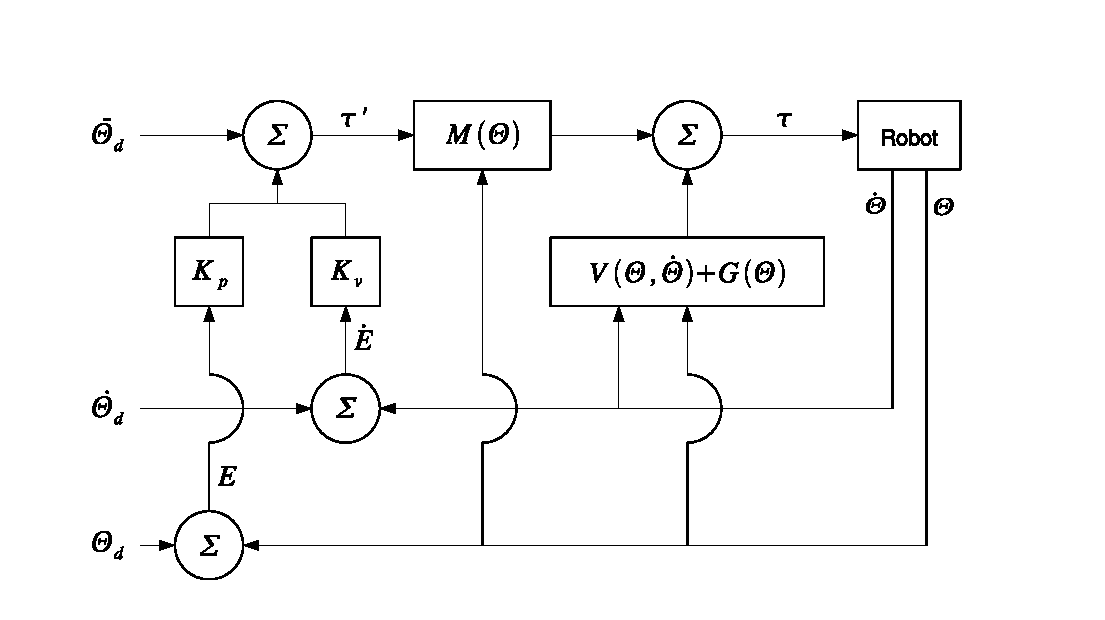
\includegraphics[width=0.5\columnwidth]{imgs/control_model-based_nonlinear.pdf}
\end{figure}

\subsection{Creating a nonlinear PD controller (Manipulator)}
\begin{enumerate}
	\item Compute $\tau$ (Dynamics)
	\item $\tau = \alpha \tau' + \beta$, \\
	where $\alpha = M(\Theta), f' = \ddot \theta$ and $\beta = V(\Theta, \dot \Theta) + G(\Theta)$
	\item $E = \theta_d - \theta$
	\item $\tau' = \ddot \theta_d + K_v \dot E + K_p E \iff \ddot E + K_v \dot E + K_p E = 0$
	\item $k_{vi} = 2 \sqrt{k_{pi}}$ (critically damped)
\end{enumerate}

\subsection{Natural frequency}
Let $k_{pi}$ be a gain.\\
The natural frequency in the context of manipulator control is computed as:
$$
	\omega_{ni} = \sqrt{k_{pi}}
$$

\section{Other Basics}

\subsection{Joint axis vectors}
$$
\hat{X} = \vect{1 \\ 0 \\ 0}
\text{,\tab}
\hat{Y} = \vect{0 \\ 1 \\ 0}
\text{,\tab}
\hat{Z} = \vect{0 \\ 0 \\ 1}
$$

\subsection{Right-Hand Coordinate System}
\begin{figure}[H]
	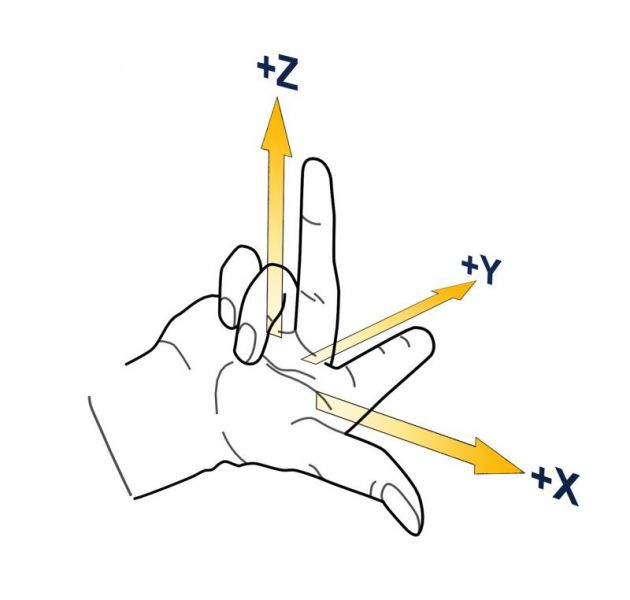
\includegraphics[width=0.5\columnwidth]{imgs/hand_xyz.jpg}
\end{figure}

\subsection{Schematic notation}

\subsubsection{Parallel axes}
Double hash marks on a simple schematic notation indicate that the axis are mutually parallel
\begin{figure}[H]
	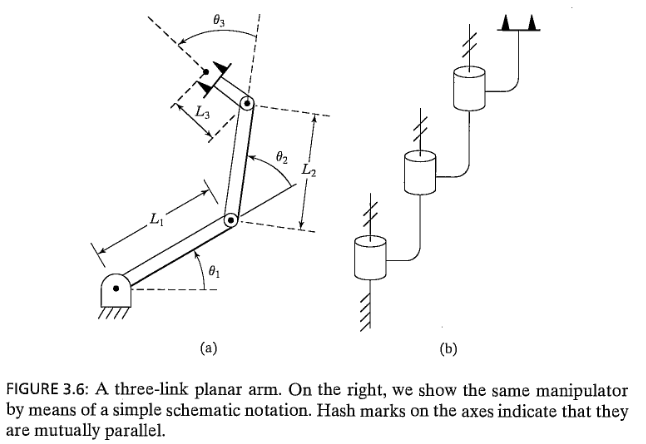
\includegraphics[width=0.5\columnwidth]{imgs/3R_arm.png}
\end{figure}

\subsubsection{orthogonal axes}




\section{Mathematical Basics}
\subsection{Rotation Matrix}
\textbf{Rotation about x-axis:}
$R_x(\theta) = \begin{bmatrix}
1 & 0 & 0 \\
0 & \cos \theta & -\sin \theta \\
0 & \sin \theta & \cos \theta 
\end{bmatrix}$ \\
\\

\textbf{Rotation about y-axis:}
$R_y(\theta) = \begin{bmatrix}
\cos \theta & 0 & \sin \theta \\
0 & 1 & 0 \\
-\sin \theta & 0 & \cos \theta
\end{bmatrix}$ \\
\\

\textbf{Rotation about z-axis:}
$R_z(\theta) = \begin{bmatrix}
\cos \theta & -\sin \theta & 0 \\
\sin \theta & \cos \theta & 0 \\
0 & 0 & 1
\end{bmatrix}$ \\
\\

\textbf{Determinant:}
$\det R = +1$

\subsection{Crossproduct}
Let $a = \vect{a_1 \\ a_2 \\ a_3}$ and $b = \vect{b_1 \\ b_2 \\ b_3}$ be two vectors. \\
The cross product is computed as:
$$
a \times b = \vect{a_1 \\ a_2 \\ a_3} \times \vect{b_1 \\ b_2 \\ b_3} = \vect{a_2b_3 - a_3b_2 \\ a_3b_1 - a_1b_3 \\ a_1b_2 - a_2b_1}
$$

\subsection{Trigonometric Functions}

\subsubsection{Arcustangens 2}
$\atan(y,x) = \begin{cases}
\arctan (\frac y x) & \text{if } x > 0 \\
\arctan (\frac y x) + \pi & \text{if } x < 0 \text{ and } y > 0 \\
\pm \pi & \text{if } x < 0 \text{ and } y = 0 \\
\arctan (\frac y x) - \pi & \text{if } x < 0 \text{ and } y < 0 \\
+ \frac \pi 2 & \text{if } x = 0 \text{ and } y > 0 \\
- \frac \pi 2 & \text{if } x = 0 \text{ and } y < 0 \\
\text{undefined} & \text{if } x = 0 \text{ and } y = 0 \\
\end{cases}$

\subsubsection{Simplifications}
$$
\cos(\alpha + \beta) = \cos \alpha ⋅ \cos \beta - \sin \alpha ⋅ \sin \beta
$$
$$
\sin(\alpha + \beta) = \sin \alpha ⋅ \cos \beta + \cos \alpha ⋅ \sin \beta
$$

\renewcommand{\arraystretch}{2}
\subsubsection{Sine, Cosine, and Tangent table}
$\begin{array}{l|ccccccccc}
\theta & 0° & 30° & 45° & 60° & 90° & 120° & 135° & 150° & 180° \\% & 210° & 240° & 270° & 300° & 330° & 360° \\
\hline
\hline
\sin\theta = -\sin(\theta - 180°) = -\sin(-\theta) & 0 & \frac 1 2 & \frac{\sqrt{(2)}}{2} & \frac{\sqrt{3}}{2} & 1 & \frac{\sqrt{3}}{2} & \frac{\sqrt{(2)}}{2} & \frac 1 2 & 0 \\
\cos\theta = -\cos(\theta - 180°) = \cos(-\theta) & 1 & \frac{\sqrt{(3)}}{2} & \frac{\sqrt{2}}{2} & \frac 1 2 & 0 & - \frac 1 2 & -\frac{\sqrt{2}}{2} & -\frac{\sqrt{(3)}}{2} & -1 \\
\tan\theta = \tan(\theta - 180°) = -\tan(-\theta) & 0 & \frac{\sqrt{3}}{3} & 1 & \sqrt{3} & \pm∞ & -{\sqrt{3}} & -1 & -\frac{\sqrt{3}}{3} & 0
\end{array}$

\renewcommand{\arraystretch}{1}

\section{Notations}
\subsection{CoSinus}
$$
\cos \theta_i ≡ c\theta_i ≡ c_i \text{\tab for } i \in \mathbb{N}
$$
$$
\sin \theta_i ≡ s\theta_i ≡ s_i \text{\tab for } i \in \mathbb{N}
$$

\subsection{CoSinus2}
$$
c_{12} = c_1c_2 - s_1s_2 = \cos(\theta_1 + \theta_2)
$$
$$
s_{12} = c_1s_2 + s_1c_2 = \sin(\theta_1 + \theta_2)
$$

\subsection{CoSinus3}
$$
c_{123} = c_1s_2s_3 + s_1s_2c_3 - s_1c_2s_3 - c_2c_3c_4
$$
$$
s_{123} = s_1c_2c_3 + c_1c_2s_3 - c_1s_2c_3 - s_1s_2s_3
$$

\pagebreak
\section*{Note}
This is a short summary of the lecture Robotics of the Technical University Munich.
This lecture was presented by Burschka D. in the winter semester 2018/19.
This summary was created by Gaida B.
All provided information is without guarantee.

\section*{References}
John J. Craig. \textit{Introduction to Robotics Mechanics and Control}. Pearson Education, Inc. New York. 2005


\end{document}








